\section{Introduction}
\label{sec:intro}

A common goal in digital simulations of life is to induce the emergence of
certain structures or processes. These might include self-replicating or
autopoietic organisms, evolutionary processes, and intelligent behavior. Often
identifying the growth of these structures and processes is reduced to
identifying a growth in complexity. Hence, designers of artificial life
simulations are interested in the question of measuring complexity.

As artificial life simulations scale, quantitatively assessing the simulation's
success in meeting the designer's criteria is essential.  Identifying and
selecting amongst the design choices of a given simulation in a qualitative
manner is not scalable and likely to admit experimental bias. As an analogy,
imagine constructing a machine-learning model to learn a given task without an
objective function. Curiosity driven exploration and reinforcement learning can
result in the model learning to successfully complete the task.  However, from
the empiricists perspective, assessing the ability of the model at completing
the task is critical. At the very least, some criterion is needed for
evaluating the model, if not training it. Similarly, in artificial life, while
the measure of complexity is typically not used as an objective to guide the
active simulation, it is at least essential to evaluate the post hoc success of
the simulation.

Complexity is notoriously ill-defined, subjective, and difficult to measure
quantitatively~\citep{gell2002complexity, mitchell2009complexity,
wiesner2019measuring}. One of the challenges in measuring complexity is
identifying the ``Goldilocks zone'' between total order and total disorder
where complexity may reside (\emph{c.f.}
figure~\ref{fig:complexity_and_entropy}). Information theoretic measures such
as Shannon entropy~\citep{shannon1948} and Kolmogorov complexity (sometimes
called Algorithmic Information Content)~\citep{kolmogorov1965, solomonoff1964},
are actually measures of randomness. As figure~\ref{fig:complexity_and_entropy}
illustrates, these measures increase monotonically with the disorder of a
system.

\begin{figure}
\centering
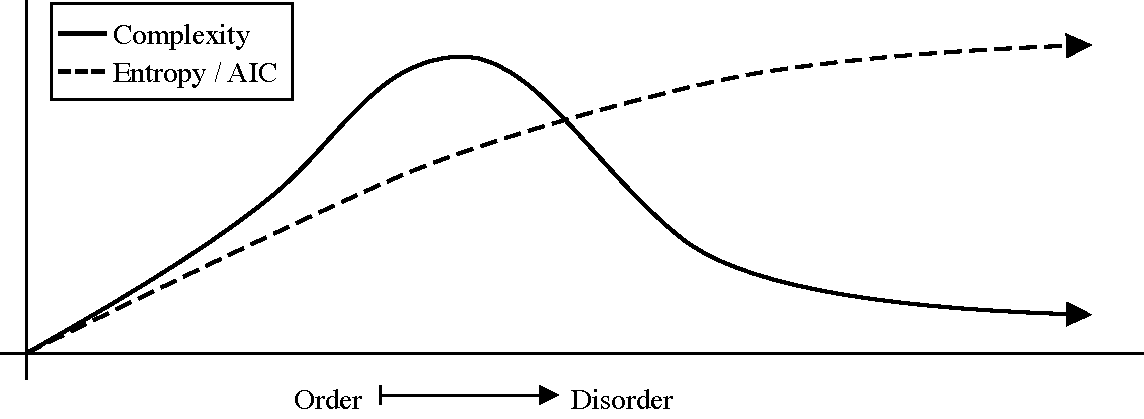
\includegraphics[width=0.7\textwidth]{figures/complexity_and_entropy}
\caption{An illustration of the one-hump of complexity (solid line) between
order and disorder. Measures such as Shannon entropy or algorithmic
information content (AIC) (both illustrated by the dashed line) grow
monotonically with disorder.}
\label{fig:complexity_and_entropy}
\end{figure}

Because of this difficulty, many measures of complexity have been
proposed~\citep{lloyd2001measures}, all with differing trade-offs. Often they
fail the ``one-hump'' criterion~\citep{adami2002complexity} increasing with
order or disorder. This is typical of the aforementioned information theoretic
criteria (Shannon entropy and Kolmogorov complexity) and constructions which
use them~\citep{lloyd1988complexity}. Other measures which satisfy the one-hump
test are not easily made operational requiring either a large degree of
subjective input from the designer or are exceedingly difficult to
compute~\citep{crutchfield1989inferring, gell1996information,
grassberger1986toward}.

We propose yet another a measure complexity, Hierarchical Information Content
(HIC). The central tenet of HIC is that complexity growth is found at the
compositions of ordered and disordered systems. We elaborate and defend the
motivating principles of HIC in section~\ref{sec:finding_complexity}. We do not
intend for HIC to serve as an ersatz for complexity in a general sense, and in
fact we make make no further attempt to rigorously define complexity. Rather,
we propose HIC as a measure which quantitatively captures some of the essential
aspects of complex systems. We promptly disclose two limitations of HIC. First,
HIC is not intended to work well for every case, but to work well for many
cases that are of interest, particularly in simulations of artificial life.
Second, while HIC can be used with few assumptions, in many instances it may
gain utility from the subjective input by the designer of the system.
